\documentclass{article}
\usepackage[utf8x]{inputenc}
\usepackage{ucs}
\usepackage{amsmath} 
\usepackage{amsfonts}
\usepackage{marvosym}
\usepackage{wasysym}
\usepackage{upgreek}
\usepackage[english,russian]{babel}
\usepackage{graphicx}
\usepackage{float}
\usepackage{textcomp}
\usepackage{hyperref}
\usepackage{geometry}
  \geometry{left=2cm}
  \geometry{right=1.5cm}
  \geometry{top=1cm}
  \geometry{bottom=2cm}
\usepackage{tikz}
\usepackage{ccaption}
\usepackage{multicol}

\hypersetup{
   colorlinks=true,
   citecolor=blue,
   linkcolor=black,
   urlcolor=blue
}

\usepackage{listings}
%\setlength{\columnsep}{1.5cm}
%\setlength{\columnseprule}{0.2pt}

\usepackage[absolute]{textpos}

\usepackage{colortbl,graphicx,tikz}
\definecolor{X}{rgb}{.5,.5,.5}


\begin{document}
\pagenumbering{gobble}
\lstdefinestyle{myCustomCStyle}{
  language=C,
  basicstyle=\linespread{1.1}\ttfamily,
  columns=fixed,
  fontadjust=true,
  basewidth=0.5em,
  keywordstyle=\color{blue}\bfseries,
  commentstyle=\color{gray},
  stringstyle=\ttfamily\color{orange!50!black},
  showstringspaces=false,
  numbersep=5pt,
  numberstyle=\tiny\color{black},
  numberfirstline=true,
  stepnumber=1,   
  numbersep=10pt,
  backgroundcolor=\color{white},
  showstringspaces=false,
  captionpos=b,
  breaklines=true,
  breakatwhitespace=true,
  xleftmargin=.2in,
  extendedchars=\true,
  keepspaces = true,
  upquote = true,
  emph = {size_t},
  emphstyle={\color{blue}\bfseries},
}


\lstdefinestyle{specialStyle}{
  style=myCustomCStyle,
  framexleftmargin=5mm, 
  frame=shadowbox, 
  rulesepcolor=\color{gray}
}

\lstset{style=myCustomCStyle}
\lstset{literate=%
   *{0}{{{\color{red!20!violet}0}}}1
    {1}{{{\color{red!20!violet}1}}}1
    {2}{{{\color{red!20!violet}2}}}1
    {3}{{{\color{red!20!violet}3}}}1
    {4}{{{\color{red!20!violet}4}}}1
    {5}{{{\color{red!20!violet}5}}}1
    {6}{{{\color{red!20!violet}6}}}1
    {7}{{{\color{red!20!violet}7}}}1
    {8}{{{\color{red!20!violet}8}}}1
    {9}{{{\color{red!20!violet}9}}}1
}
\renewcommand{\thesubsection}{\arabic{subsection}}
\makeatletter
\def\@seccntformat#1{\@ifundefined{#1@cntformat}%
   {\csname the#1\endcsname\quad}%    default
   {\csname #1@cntformat\endcsname}}% enable individual control
\newcommand\section@cntformat{}     % section level 
\newcommand\subsection@cntformat{Задача \thesubsection.\space} % subsection level
\newcommand\subsubsection@cntformat{\thesubsubsection.\space} % subsubsection level
\makeatother
\title{Семинар \#6: Динамический массив. Домашнее задание.\vspace{-5ex}}\date{}\maketitle

\subsection{Новые функции для динамического массива}
В папке \texttt{dynarray} лежит реализация динамического массива. Вам нужно написать ещё несколько функций для работы с этим динамическим массивом и протестировать их. Функции нужно написать в файле \texttt{dynarray.h}, а код для тестирования в файле \texttt{main.c}.



\subsubsection{\texttt{\textcolor{blue}{int} pop\_back(Dynarray* pd)}}
Функция должна будет удалять последний элемент массива и возвращать его. Вместимость массива в этой функции меняться не должна.


\subsubsection{\texttt{\textcolor{blue}{void} resize(Dynarray* pd, \textcolor{blue}{size\_t} new\_size)}}
Функция должна будет изменять размер массива на \texttt{new\_size}. Если \texttt{new\_size} будет меньше, чем старый размер, то размер массива должен уменьшиться. При увеличении размера новые элементы массива должны быть равны нулю.


\subsubsection{\texttt{\textcolor{blue}{void} shrink\_to\_fit(Dynarray* pd)}}
Функция должна делать вместимость массива равной её размеру.\\
\begin{center}
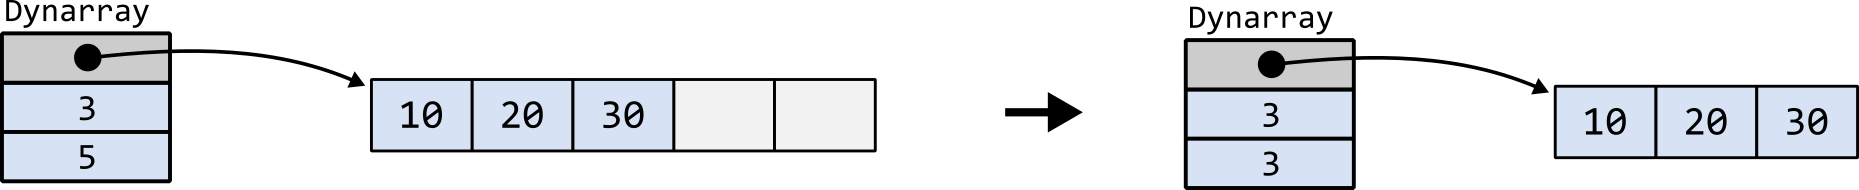
\includegraphics[scale=1]{../images/dynarray_shrink_to_fit.png}
\end{center}

\subsubsection{Поверхностная копия: \texttt{Dynarray shallow\_copy(Dynarray* pd)}}
Создаёт поверхностную копию динамического массива. При поверхностном копировании копируется только сам объект, а все ресурсы, связанные с этим объектом не копируются.
\begin{center}
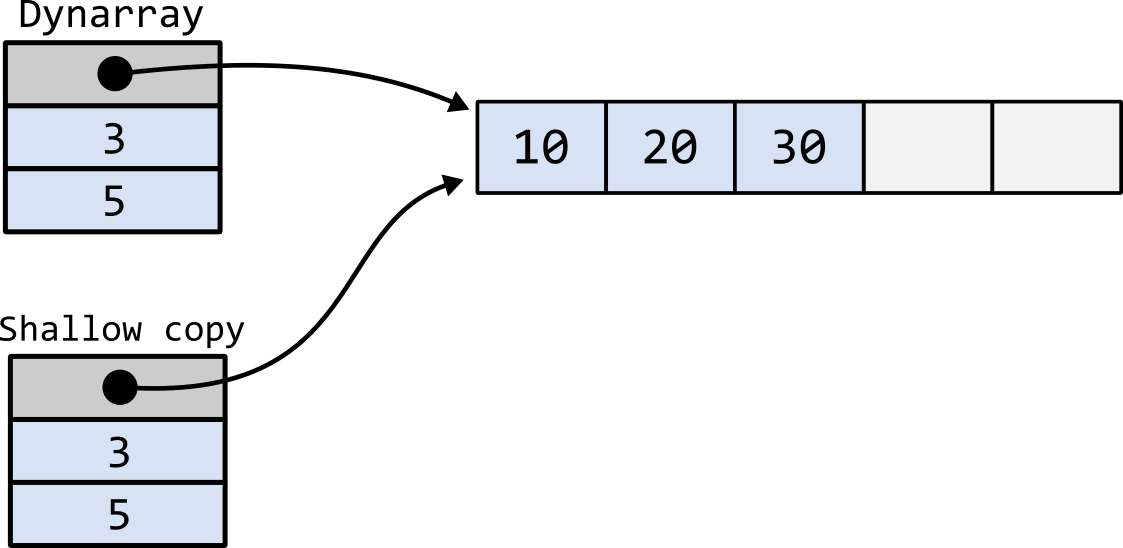
\includegraphics[scale=0.8]{../images/dynarray_shallow.png}
\end{center}

\subsubsection{Глубокая копия: \texttt{Dynarray deep\_copy(const Dynarray* pd)}}
Создаёт глубокую копию динамического массива. При глубоком копировании копируется и сам объект и все ресурсы, связанные с этим объектом.
\begin{center}
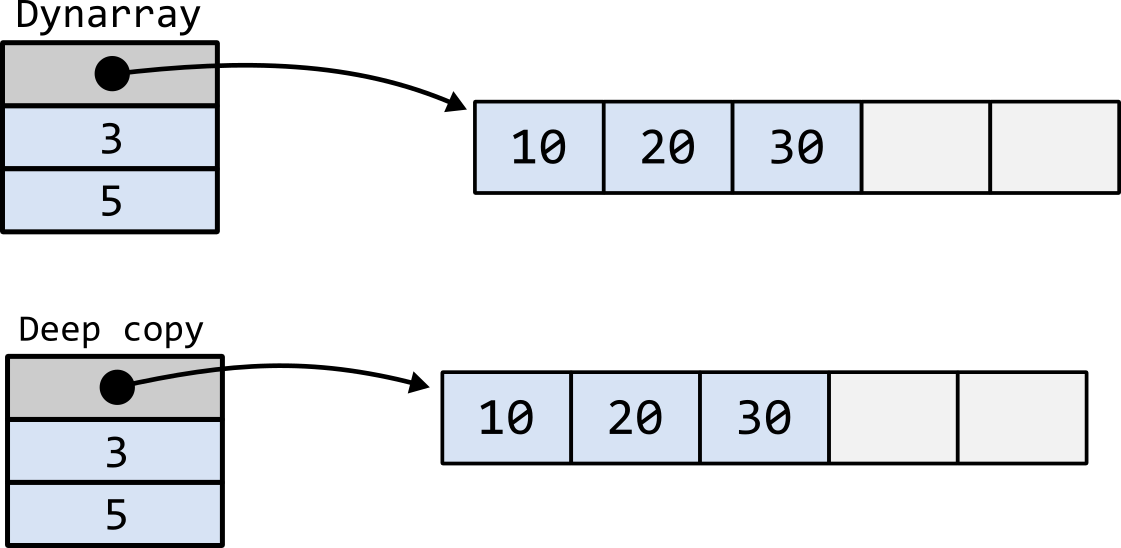
\includegraphics[scale=0.8]{../images/dynarray_deep.png}
\end{center}

\newpage
\subsection{Двусвязный список}
Напишите свою реализацию структуры данных двусвязный список, хранящий элементы типа \texttt{int}.
Узел такого списка будет выглядеть так:
\begin{lstlisting}
struct node 
{
    int value;
    struct node* next;
    struct node* prev;
};
typedef struct node Node;
\end{lstlisting}
Структура для самого двусвязного списка и расположение двусвязного списка в памяти:\\

\noindent\begin{minipage}{.35\textwidth}
\begin{lstlisting}
struct list 
{
    Node* head;
    Node* tail;
    size_t size;
};
typedef struct list List;
\end{lstlisting}
\end{minipage}
\begin{minipage}{.55\textwidth}
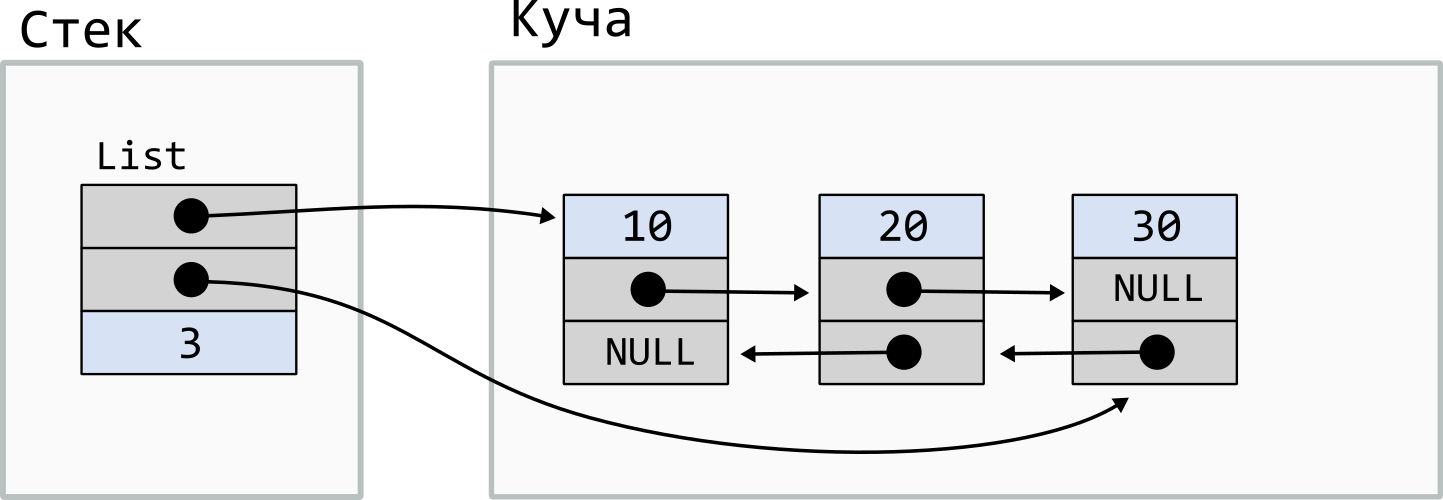
\includegraphics[scale=0.8]{../images/list.png}
\end{minipage}

Поля структуры \texttt{List}:
\begin{itemize}
\item \texttt{head} -- указатель на первый узел двусвязного списка
\item \texttt{tail} -- указатель на последний узел двусвязного списка
\item \texttt{size} -- количество элементов в двусвязном списке
\end{itemize}
Вам нужно будет написать и протестировать следующие функции для работы с двусвязным списком.
Реализация списка должна находиться в файле \texttt{list.h}. Это файл должен подключаться к файлу \texttt{main.c}, в котором и должно происходить тестирование списка.

\subsubsection{\texttt{List init(\textcolor{blue}{size\_t} n)}}
Возвращает двусвязный список из \texttt{n} нулевых элементов. Если \texttt{n} равно нулю, то возвращает пустой двусвязный список, который должен выглядеть вот так:
\begin{center}
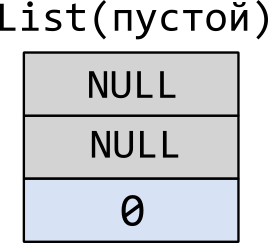
\includegraphics[scale=1]{../images/list_empty.png}
\end{center}

\subsubsection{\texttt{\textcolor{blue}{void} print(\textcolor{blue}{const} List* pl)}}
Печатает все элементы списка.

\subsubsection{\texttt{\textcolor{blue}{void} push\_back(List* pl, \textcolor{blue}{int} value)}}
Добавляет элемент в конец списка.

\subsubsection{\texttt{\textcolor{blue}{int} pop\_back(List* pl)}}
Удаляет элемент из конца списка и возвращает его.

\subsubsection{\texttt{\textcolor{blue}{void} push\_front(List* pl, \textcolor{blue}{int} value)}}
Добавляет элемент в начало списка.

\subsubsection{\texttt{\textcolor{blue}{int} pop\_front(List* pl)}}
Удаляет элемент из начала списка и возвращает его.

\iffalse
\subsubsection{\texttt{\textcolor{blue}{void} insert(List* pl, Node* p, \textcolor{blue}{int} value)}}
Указатель \texttt{p} указывает на один из узлов списка.
Функция должна вставлять новый элемент со значением \texttt{value} до элемента, на узел которого указывает \texttt{p}.
\fi

\subsubsection{\texttt{Node* erase(List* pl, Node* p)}}
Указатель \texttt{p} указывает на один из узлов списка.
Функция должна удалять узел, на который указывает \texttt{p}, и возвращать указатель на узел, следующий после удалённого. В случае удаления последнего узла функция должна возвращать \texttt{NULL}.


\subsubsection{\texttt{\textcolor{blue}{void} splice(List* plist, Node* p, List* pother)}}
Переносит все элементы из списка на который указывает \texttt{pother} в список на который указывает \texttt{plist}. Новые элементы должны быть вставлены сразу перед узлом на который указывает \texttt{p}. Порядок элементов не должен измениться. После выполнения этой операции список на который указывает \texttt{pother} должен стать пустым.

\subsubsection{\texttt{\textcolor{blue}{void} destroy(List* pl)}}
Удаляет все элементы списка и зануляет все поля структуры \texttt{List}.


\subsubsection{\texttt{\textcolor{blue}{void} advance(Node** pp, size\_t n)}}
Функция должна принимать адрес указателя на один из узлов связного списка и изменяет этот указатель так, чтобы он указывал на \texttt{n} узлов вперёд. Если количество узлов до конца списка меньше, чем \texttt{n} то функция должна изменить значение указателя на \texttt{NULL}. 


\subsubsection{Тестирование}
Протестируйте вашу реализацию списка, используя следующий код:
\begin{lstlisting}
#include <stdio.h>
#include "list.h"
int main()
{
    List a = init(0);
    
    for (int i = 0; i < 5; ++i)
        push_back(&a, 10 * (i + 1));
    for (int i = 0; i < 5; ++i)
        push_front(&a, 100 * (i + 1));
    print(&a);                          // Напечатает 500 400 300 200 100 10 20 30 40 50
                                        //                
    printf("%i\n", pop_front(&a));      // Напечатает 500
    printf("%i\n", pop_back(&a));       // Напечатает 50
    print(&a);                          // Напечатает 400 300 200 100 10 20 30 40
                                        //            
    Node* p = a.head;                   //     
    advance(&p, 3);                     //
    p = erase(a, p);                    //
    print(&a);                          // Напечатает 400 300 200 10 20 30 40
                                        //            
    List b = init(0);                   //
    for (int i = 0; i < 3; ++i)         //
        push_back(&a, 1000 * (i + 1));  //
    splice(&a, p, &b);                  //
                                        //
    print(&a);                          // Напечатает 400 300 200 1000 2000 3000 10 20 30 40
    print(&b);                          // Ничего не напечатает
}

\end{lstlisting}


\subsection{Счет}
Напишите программу, которая будет вести себя по-разному в зависимости от того какая опция была передана при компиляции. Программа должна печатать числа от \texttt{1} до значения передаваемого на этапе компиляции макроса \texttt{COUNT}.
То есть, если скомпилировать программу так:
\begin{verbatim}
    gcc -DCOUNT=5 main.c
\end{verbatim}
то программа при запуске должна напечатать числа от \texttt{1} до \texttt{5}:
\begin{verbatim}
    1 2 3 4 5
\end{verbatim}
В случае же если опции \texttt{-DCOUNT} при компиляции программы передано не было, например при такой компиляции:
\begin{verbatim}
    gcc main.c
\end{verbatim}
программа при запуске должна напечатать:
\begin{verbatim}
    No Count!
\end{verbatim}

\newpage


\section*{Необязательные задачи (не входят в ДЗ, никак не учитываются)}
\setcounter{subsection}{0}
\subsection{Очередь}
\begin{multicols}{2}
\begin{lstlisting}
#define CAPACITY 7
typedef int Data;

struct queue
{
    int front;
    int back;
    Data values[CAPACITY];
};
typedef struct queue Queue;

// ......

int main()
{
    Queue a;
    queue_init(&a);
    enqueue(&a, 100);
    for (int i = 0; i < 20; ++i)
    {
        enqueue(&a, i);
        dequeue(&a);
    }
    enqueue(&a, 200);
    queue_print(&a);
}
\end{lstlisting}
\vfill\null
Очередь — абстрактный тип данных с дисциплиной доступа к элементам «первый пришёл — первый вышел». \\
Реализация с помощью массива:
\begin{center}
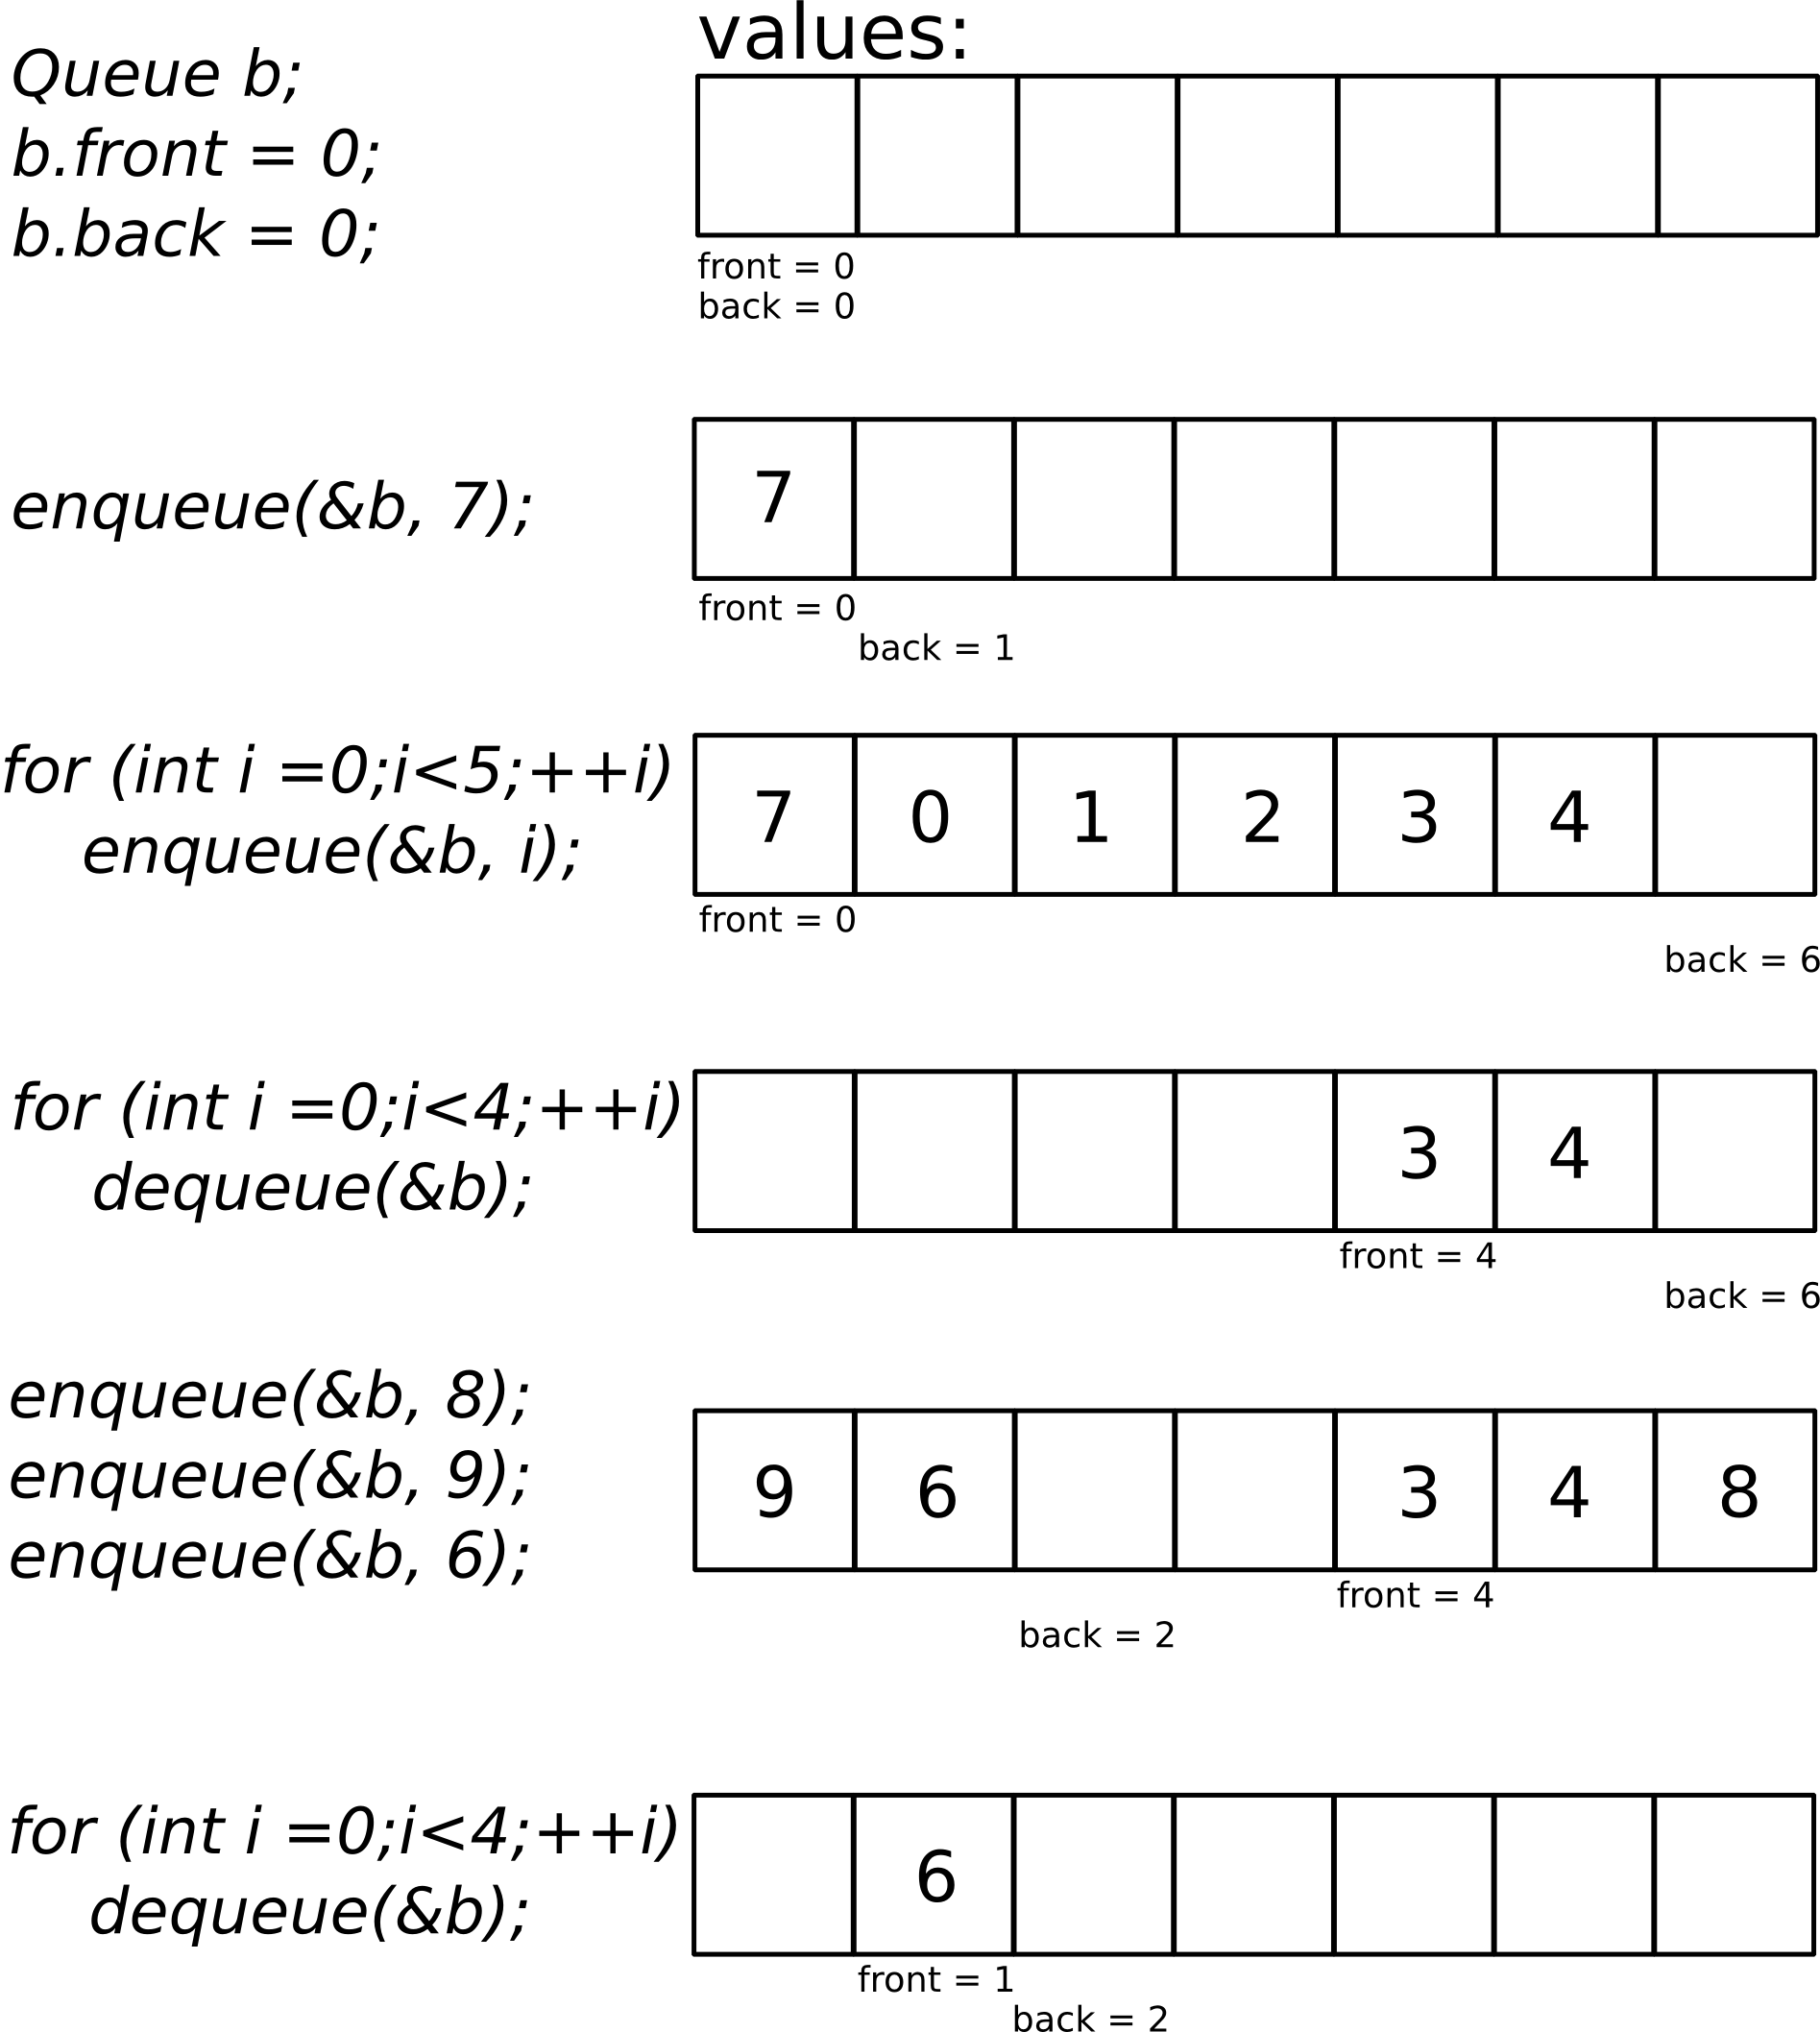
\includegraphics[width=1.05\linewidth]{../images/queue.png}
\end{center}
\end{multicols}

\textbf{Задача \#3: Очередь на основе статического массива}:
\begin{enumerate}
\item Написать функцию \texttt{void queue\_init(Queue* q)}, которая будет задавать начальные значения полей \texttt{front} и \texttt{back}.
\item Написать функцию \texttt{void enqueue(Queue* q, Data x)} - добавляет \texttt{x} в очередь. Для эффективной реализации очереди, нужно использовать как можно меньше операций и как можно эффективней использовать выделенную память. Поэтому, при заполнении массива, если начало массива свободно, то элементы можно хранить там. (смотрите рисунок)
\item Написать функцию \texttt{Data dequeue(Queue* q)} - удаляет элемент из очереди и возвращает его. Для  эффективной реализации очереди сдвигать оставшиеся элементы не нужно. Вместо этого можно просто увеличить поле \texttt{front}.
\item Написать функцию \texttt{int queue\_is\_empty(const Queue* q)}, которая возвращает \texttt{1} если очередь пуста и \texttt{0} иначе.
\item Написать функцию \texttt{int queue\_get\_size(const Queue* q)}, которая возвращает количество элементов.
\item Написать функцию \texttt{int queue\_is\_full(const Queue* q)}, которая возвращает \texttt{1} если очередь заполнена и \texttt{0} иначе. Очередь считается полной, если \texttt{size == capacity - 1}.
\item Написать функции \texttt{Data queue\_get\_front(const Queue* q)} и \texttt{Data queue\_get\_back(const Queue* q)}, которые возвращают элементы, находящиеся в начале и в конце очереди соответственно, но не изменяют очередь.
\item Написать функцию \texttt{void queue\_print(const Queue* q)}, которая распечатывает все элементы очереди.
\item Что произойдёт, если вызвать \texttt{enqueue} при полной очереди или \texttt{dequeue} при пустой? Обработайте эти ситуации. Программа должна печатать сообщение об ошибке и завершаться с аварийным кодом завершения. Чтобы завершить программу таким образом можно использовать функцию \texttt{exit} из библиотеки \texttt{stdlib.h}.

\item Протестируйте очередь на следующих тестах:
\begin{enumerate}
\item В очередь добавляется 4 элемента, затем удаляется 2. Вывести содержимое очереди с помощью \texttt{queue\_print()}
\item В очередь добавляется очень много элементов (больше чем \texttt{CAPACITY}). Программа должна напечатать сообщение об ошибке.
\item В очередь добавляется 3 элемента, затем удаляется 2, затем добавляется очень много элементов (больше чем \texttt{CAPACITY}). Программа должна напечатать сообщение об ошибке.
\item В очередь добавляется 3 элемента, затем удаляется 4. Программа должна напечатать сообщение об ошибке.
\item В очередь добавляется 2 элемента, затем выполняется следующий цикл:
\begin{verbatim}
for (int i = 0; i < 10000; ++i)
{
    enqueue(&a, i);
    dequeue(&a);
}
\end{verbatim}
Вывести содержимое очереди с помощью \texttt{queue\_print()}
\end{enumerate}
\end{enumerate}

\textbf{Задача \#4: Очередь на основе динамического массива}:

Описание такой очереди выглядит следующим образом:
\begin{lstlisting}
struct queue
{
    int capacity;
    int front;
    int back;
    Data* values;
};
typedef struct queue Queue;
\end{lstlisting}

\begin{enumerate}
\item Скопируйте код очереди со статическим массивом в новый файл и измените описание структуры как показано выше. Макрос \texttt{CAPACITY} больше не нужен, его можно удалить.

\item Измените функцию \texttt{void queue\_init(Queue* q)} на \texttt{void queue\_init(Queue* q, int initial\_capacity)}. Теперь она должна присваивать \texttt{capacity} начальное значение \texttt{initial\_capacity} и выделять необходимую память под массив \texttt{values}.

\item Измените функцию \texttt{void enqueue(Queue* q)}. Теперь, при заполнении очереди должно происходить перевыделение памяти с помощью функции \texttt{realloc}. Заполнение очереди достигается когда размер очереди становится равным \texttt{capacity - 1} (а не \texttt{capacity}, потому что при полном заполнении вместимости \texttt{front} будет равняться \texttt{back} и мы не сможем понять полная эта очередь или пустая).
После перевыделения нужно переместить элементы массива на новые места и изменить \texttt{front} и \texttt{back}. Если \texttt{front != 0}, то нужно переместить элементы массива от \texttt{front} до конца старого массива \texttt{values} в конец нового массива \texttt{values}. (смотрите рисунок ниже)

\item Добавьте функцию \texttt{void queue\_destroy(Queue* q)}, которая будет освобождать память, выделенную под массив \texttt{values}.

\item Протестируйте очередь: в очередь добавляется много элементов ($\gg 10^3 >$ \texttt{initial\_capacity}). Программа \textbf{не} должна напечатать сообщение об ошибке (если только совокупный размер элементов не превышает размер доступной оперативной памяти). 

\item В случае, если \texttt{malloc} или \texttt{realloc} не смогли выделить запрашиваемый объём памяти (например, по причине того, что этот объём  больше, чем вся доступная оперативная память или по какой-нибудь иной причине), то они возвращают значение \texttt{NULL}. Программа должна это учитывать и завершаться с ошибкой, если нельзя выделить нужный объём памяти.
\end{enumerate}

\subsection*{Схема перевыделения памяти для очереди на основе динамического массива:}
Очередь будет считаться заполненной: 
\begin{itemize}
\item Если \texttt{front == 0}, а \texttt{back == capacity - 1}
\item Или если \texttt{front != 0}, а \texttt{front - back == 1}. (А не \texttt{front - back == 0}, потому что при полном заполнении вместимости \texttt{front} будет равняться \texttt{back} и мы не сможем понять полная эта очередь или пустая).
\end{itemize}
 Когда очередь заполнена и мы хотим добавить в неё ещё один элемент, то её нужно увеличить. Делается это так, как представлено на схеме ниже:
\begin{center}
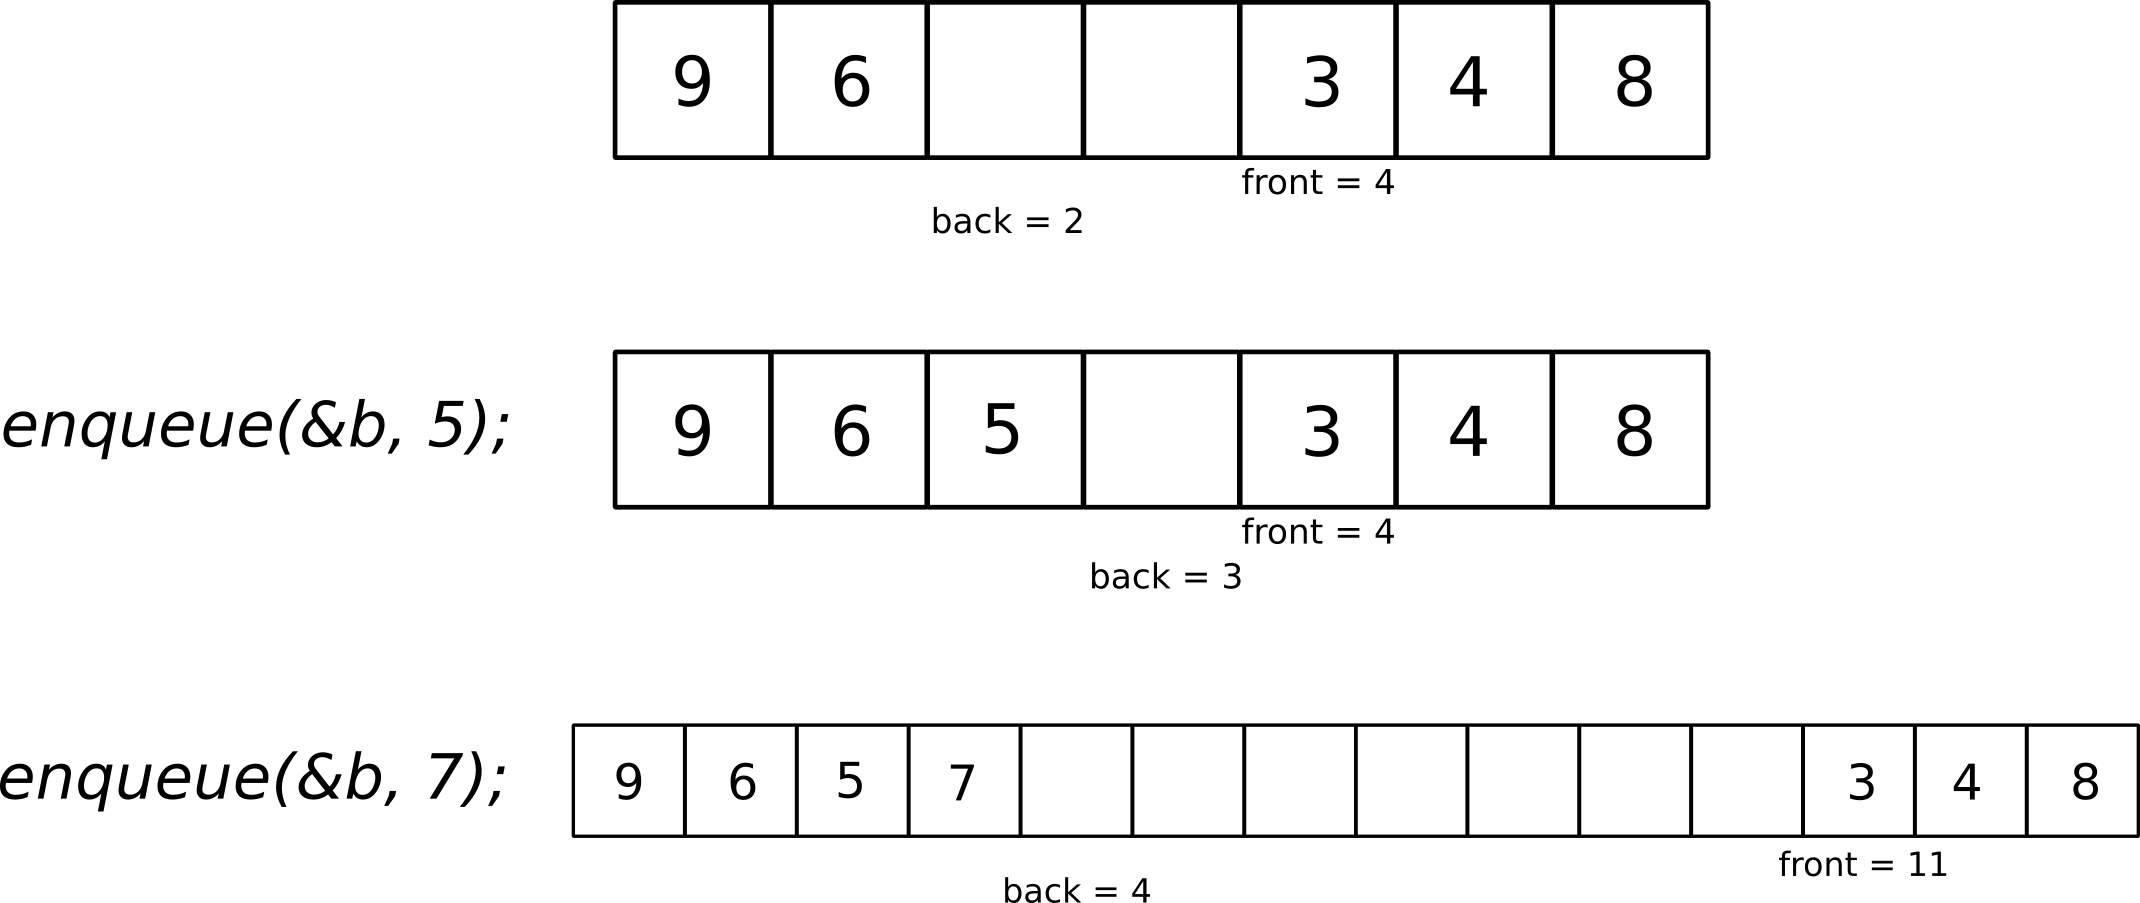
\includegraphics[scale=0.8]{../images/queue_dynamic.png}
\end{center}

\begin{itemize}
\item Если \texttt{front == 0}, то нужно просто увеличить очередь с помощью \texttt{realloc}.
\item Если \texttt{front != 0}, то нужно ещё и перекопировать хвост очереди в конец и изменить \texttt{front}.
\end{itemize}
\end{document}